% =====================================================================
% ICONIP submission version (Springer LNCS)
% Project: DimASQP-Refine — Dimensional Aspect Sentiment Quad Prediction
% Author : Hongzhen Qin (Yamanashi University)
%
% Build:   pdflatex paper_draft_iconip.tex
% Reqs:    llncs.cls and splncs04.bst from Springer:
%          https://www.springer.com/gp/computer-science/lncs/conference-proceedings-guidelines
% =====================================================================
\documentclass[runningheads]{llncs}

\usepackage[T1]{fontenc}
\usepackage{graphicx}
\usepackage{amsmath,amssymb}
\usepackage{booktabs}
\usepackage{multirow}
\usepackage{url}
\usepackage{xcolor}
\usepackage{enumitem}
\usepackage{hyperref}

% ----- TikZ for the architecture figure -----
\usepackage{tikz}
\usetikzlibrary{positioning, arrows.meta, shapes.geometric,
                fit, backgrounds, calc, decorations.pathreplacing}
\tikzset{
  block/.style    ={rectangle, rounded corners=2pt, draw=black!70,
                    fill=white, align=center, font=\scriptsize,
                    minimum height=6.5mm, inner sep=2pt},
  encblock/.style ={block, fill=blue!8,  draw=blue!50},
  headblock/.style={block, fill=green!8, draw=green!55!black},
  rethink/.style  ={block, fill=orange!12, draw=orange!75!black},
  outblock/.style ={block, fill=gray!10, draw=black!60,
                    minimum height=7mm},
  flow/.style     ={-{Stealth[length=1.6mm]}, thick, draw=black!75},
  dashflow/.style ={-{Stealth[length=1.6mm]}, thick, dashed,
                    draw=orange!80!black},
  tag/.style      ={font=\scriptsize\itshape, text=black!55, inner sep=1pt}
}

% LNCS uses numerical citations by default; \cite{key} is enough.

\begin{document}

\title{Draft-then-Refine with Multi-Source Transfer for\\
Dimensional Aspect Sentiment Quad Prediction}
\titlerunning{Draft-then-Refine for Dimensional ASQP}

\author{Hongzhen Qin\inst{1}}
\authorrunning{H.~Qin}
\institute{Yamanashi University, Kofu, Japan\\
\email{qhz0.0@outlook.com}}

\maketitle

\begin{abstract}
We present \textbf{DimASQP-Refine}, a system for SemEval-2026 Task~3
(Dimensional Aspect-Based Sentiment Analysis), which extends Aspect
Sentiment Quad Prediction with continuous Valence--Arousal (V--A)
intensity scores. Existing quadruple extractors are designed for
discrete polarity labels; directly transplanting them to the dimensional
setting yields severe span/category errors and biased V--A regression,
especially for low-resource languages. We propose a two-stage
\emph{Draft-then-Refine} architecture in which a Feature-level Rethink
module re-encodes the hidden states using soft label embeddings of the
draft predictions, and we couple it with Hungarian matching between
predicted and gold quads so that all heads receive a well-aligned
training signal. To address data scarcity in seven non-English
languages, we further introduce (i) multi-pivot back-translation with
COMET-based filtering, (ii) cross-lingual encoder transfer that
initialises low-resource languages from a high-resource source, and
(iii) MeCab-based span post-processing for Japanese. Combined with a
dual-layer ensemble (top-$k$ weight averaging within seeds and majority
voting across seeds), the system reaches an average $\mathrm{cF1}$ of
\textbf{0.4397} over the eight official datasets, surpassing the
Llama-3.3 70B baseline by \textbf{+5.4} absolute points and beating all
four official LLM baselines on \textbf{7/8} languages, while remaining
under 100M parameters.

\keywords{Aspect-Based Sentiment Analysis \and Valence--Arousal
\and Cross-Lingual Transfer \and Hungarian Matching \and Data
Augmentation.}
\end{abstract}

% ============================================================
\section{Introduction}
\label{sec:intro}
% ============================================================

Aspect-Based Sentiment Analysis (ABSA) has steadily moved from
single-element extraction (aspect, opinion, or polarity in isolation)
toward composite \emph{Aspect Sentiment Quad Prediction} (ASQP), in
which a system must extract every quadruple
$(a, c, o, s)$ from a review, where $a$ is an aspect term, $c$ a
category, $o$ an opinion expression, and $s$ a sentiment label.
SemEval-2026 Task~3~\cite{dimabsa2026} introduces a new
\textbf{dimensional} variant: the discrete polarity $s$ is replaced by
a continuous two-dimensional vector $(V, A) \in [1,9]^2$ taken from
Russell's circumplex model~\cite{russell1980circumplex}, where $V$
(valence) measures positivity and $A$ (arousal) measures intensity.
For example, ``\textit{The Thai food was delicious, but delivery was
terrible.}'' should produce
\begin{quote}\small
$(\text{Thai food}, \text{FOOD\#QUALITY}, \text{delicious}, 7.50\#6.20)$,\\
$(\text{delivery}, \text{SERVICE\#GENERAL}, \text{terrible}, 2.10\#7.00)$.
\end{quote}
The shared task spans \textbf{eight} datasets covering five languages
(English, Russian, Tatar, Ukrainian, Chinese, Japanese) and two domains
(restaurant, laptop, hotel), and is evaluated under a single primary
metric \emph{Continuous F1} (cF1) that simultaneously rewards
categorical correctness and V--A regression accuracy.

\paragraph{Problems we focus on.}
Although discrete-polarity ASQP is now a mature task, the dimensional
setting introduces several problems that previous systems do not
handle well:
\begin{enumerate}[itemsep=2pt,topsep=2pt,leftmargin=*]
  \item \textbf{Span--label inconsistency.} Span extractors and pair
    classifiers are typically trained independently. The classifier
    therefore receives noisy, low-recall spans during training and
    cannot recover at inference.
  \item \textbf{Pair--gold misalignment.} Models enumerate the
    Cartesian product of aspect and opinion candidates, producing far
    more pairs than there are gold quads; without an explicit
    assignment the loss is computed on the wrong correspondences.
  \item \textbf{Heavy data imbalance across languages.} The training
    set ranges from 1{,}240 sentences (rus, tat, ukr) to 6{,}050 (zho
    restaurant)---too small for low-resource languages, but too varied
    to be solved by a single off-the-shelf augmentation recipe.
  \item \textbf{Polarity-shift in synthetic data.} Standard data
    augmentation (back-translation, LLM paraphrase, pseudo-labelling)
    routinely produces sentences whose surface form preserves the
    aspect/opinion words but whose sentiment is altered, which is
    catastrophic when the target $(V, A)$ values are continuous.
\end{enumerate}

\paragraph{Contributions.}
We address the above with the following contributions:
\begin{enumerate}[itemsep=2pt,topsep=2pt,leftmargin=*]
  \item A \emph{Draft-then-Refine} model with a Feature-level Rethink
        module that injects soft embeddings of stage-1 BIO,
        category, and V--A predictions back into the encoder before
        stage-2 prediction (Section~\ref{sec:method:rethink}).
  \item Hungarian matching between predicted and gold quads as the
        loss-assignment rule, with a four-term cost combining span
        IoU, category log-likelihood, and V--A distance
        (Section~\ref{sec:method:hungarian}).
  \item A unified low-resource pipeline: multi-pivot back-translation
        with substring-based span re-localisation, cross-lingual
        encoder transfer from a high-resource source, MeCab-based
        Japanese span trimming, and a dual-layer ensemble that
        averages top-$k$ checkpoint weights within each seed before
        cross-seed voting (Section~\ref{sec:method:lowres}).
  \item A thorough study of \emph{negative} results: we report and
        analyse why CRF decoding, DeBERTa-v3-large, multi-source
        transfer (V7) and unfiltered LLM pseudo-labels (V8) all fail
        to improve over our V6 system, and how COMET filtering and
        label-preserving paraphrase (V9) are designed to remove the
        identified failure modes (Section~\ref{sec:negative}).
  \item State-of-the-art results among sub-100M-parameter systems on
        seven of the eight official datasets and the strongest
        macro-average (cF1 0.4397) reported to date, beating all
        official LLM baselines including Llama-3.3 70B and GPT-OSS
        120B (Section~\ref{sec:results}).
\end{enumerate}

% ============================================================
\section{Related Work}
\label{sec:related}
% ============================================================

\paragraph{ASQP and ACOS.}
Cai et al.~\cite{cai2021acos} introduced the four-element ASQP/ACOS
task and proposed a generation-style baseline.
Zhang et al.~\cite{zhang2021seq2path} cast quad prediction as
sequence-to-sequence path generation, while
Mao et al.~\cite{mao2022mvp} use multi-view prompting on T5.
Hu et al.~\cite{hu2022extractthenpredict} adopt a pipeline of span
extraction followed by pair classification.
All these methods optimise the four targets \emph{independently}; we
show in Section~\ref{sec:method:rethink} that re-encoding the hidden
states with the draft predictions yields a much stronger second-stage
signal.

\paragraph{Dimensional ABSA.}
Lee et al.~\cite{lee2022dimabsa} first proposed the dimensional
Valence--Arousal formulation. SIGHAN-2024~\cite{sighan2024dimabsa}
hosted a Chinese DimABSA shared task whose top systems
(HITSZ-HLT, CCIIPLab) demonstrated the importance of continued
pre-training and contrastive V--A regularisation. Our work transfers
these ideas to the multilingual SemEval-2026 setting and adds the
two-stage Rethink architecture, which is orthogonal to those
techniques.

\paragraph{Set prediction and Hungarian matching.}
DETR~\cite{carion2020detr} first popularised Hungarian matching for
set prediction in object detection; it has since been used for
relation extraction~\cite{tan2022rete} and aspect-opinion pair
extraction~\cite{chen2022spaopn}. Our cost design is novel in that it
mixes a span-level IoU term with a continuous V--A distance term, so
that the assignment is consistent with the cF1 metric.

\paragraph{Cross-lingual transfer for ABSA.}
Li et al.~\cite{li2020xabsa} use mBERT for cross-lingual ABSA via
parameter sharing.
Lin et al.~\cite{lin2023xacos} apply XLM-R for cross-lingual ACOS.
We show that for low-resource languages a much simpler
approach---warm-starting the entire model from the best Chinese
checkpoint---recovers most of the gain at almost no engineering cost.

\paragraph{Data augmentation for ABSA.}
EDA-style word substitution~\cite{wei2019eda} and
back-translation~\cite{sennrich2016bt} are the standard tools.
Li et al.~\cite{li2024llmabsa} use LLM pseudo-labelling.
Our results in Section~\ref{sec:negative} replicate the SIGHAN-2024
finding that unfiltered synthetic data hurts dimensional ABSA, and we
propose COMET-based filtering plus label-preserving paraphrasing as
counter-measures.

% ============================================================
\section{Method}
\label{sec:method}
% ============================================================

\subsection{Task formulation}
\label{sec:method:task}

Given an input sentence $x = (x_1, \dots, x_n)$, the model must output
a set of quadruples $\mathcal{Y}=\{(a_i, c_i, o_i, V_i, A_i)\}_{i=1}^k$
where $a_i$ and $o_i$ are spans of $x$ (or the special token
\textsc{null}), $c_i = (e_i, t_i)$ is a (category-entity,
category-attribute) pair, and $(V_i,A_i)\in[1,9]^2$. Cardinality $k$
is unknown a priori.

The official metric is
\begin{equation}
\mathrm{cF1} = \frac{2\, \mathrm{cP}\, \mathrm{cR}}{\mathrm{cP}+\mathrm{cR}},
\quad
\mathrm{c\!\:TP}_i = 1 - \frac{\| (V,A)_{\text{pred}} - (V,A)_{\text{gold}} \|_2}{D_{\max}},
\label{eq:cf1}
\end{equation}
where $D_{\max}=\sqrt{2\cdot 8^2}\!\approx\!11.31$ is the largest
possible Euclidean distance in the V--A square. A predicted quad
contributes a partial-credit cTP only if its categorical part
$(a, c, o)$ already matches a gold quad.

\subsection{Backbone}
\label{sec:method:backbone}

We use DeBERTa-v3-base~\cite{he2023deberta} for English and
mDeBERTa-v3-base for the seven non-English datasets. The encoder
produces contextual representations $H \in \mathbb{R}^{n\times d}$,
$d=768$. Figure~\ref{fig:arch} shows the full architecture; the
remaining subsections describe each component.

% ====================== Architecture figure ======================
\begin{figure}[t]
\centering
\resizebox{\textwidth}{!}{%
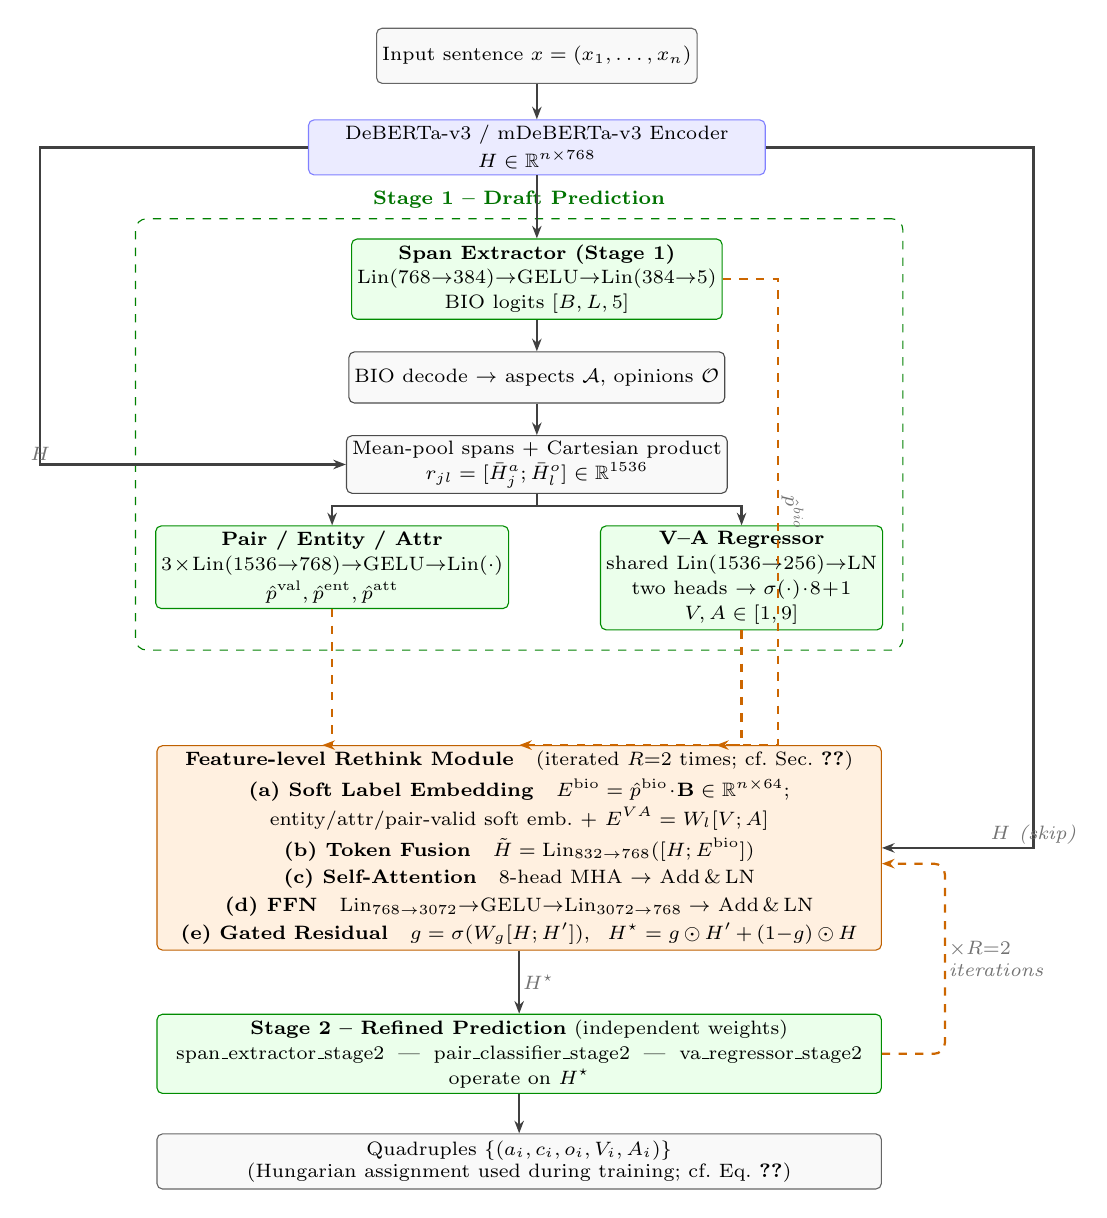
\begin{tikzpicture}[node distance=4.5mm and 6mm]

% --- Input ---
\node[outblock, fill=gray!5] (input)
  {Input sentence $x = (x_1, \dots, x_n)$};

% --- Encoder ---
\node[encblock, below=of input, minimum width=58mm] (enc)
  {DeBERTa-v3 / mDeBERTa-v3 Encoder\\[1pt]
   $H \in \mathbb{R}^{n\times 768}$};

% --- Stage-1 backbone heads ---
\node[headblock, below=8mm of enc, minimum width=44mm] (span1)
  {\textbf{Span Extractor (Stage 1)}\\[1pt]
   $\mathrm{Lin}(768{\to}384){\to}\mathrm{GELU}{\to}\mathrm{Lin}(384{\to}5)$\\[1pt]
   BIO logits $[B,L,5]$};

\node[block, below=4mm of span1, minimum width=44mm, fill=gray!5]
  (decode) {BIO decode $\to$ aspects $\mathcal{A}$, opinions $\mathcal{O}$};

\node[block, below=4mm of decode, minimum width=44mm, fill=gray!5]
  (pool)  {Mean-pool spans + Cartesian product\\[1pt]
           $r_{jl}=[\bar H^{a}_j;\bar H^{o}_l]\in\mathbb{R}^{1536}$};

\node[headblock, below=4mm of pool, xshift=-26mm, minimum width=24mm]
  (paircls) {\textbf{Pair / Entity / Attr}\\[1pt]
             $3\!\times\!\mathrm{Lin}(1536{\to}768){\to}\mathrm{GELU}{\to}\mathrm{Lin}(\cdot)$\\[1pt]
             $\hat p^\text{val},\hat p^\text{ent},\hat p^\text{att}$};

\node[headblock, below=4mm of pool, xshift=26mm, minimum width=24mm]
  (vareg)   {\textbf{V--A Regressor}\\[1pt]
             shared $\mathrm{Lin}(1536{\to}256){\to}\mathrm{LN}$\\[1pt]
             two heads $\to\sigma(\cdot)\!\cdot\!8\!+\!1$\\[1pt]
             $V,A\in[1,9]$};

% Group Stage-1 background
\begin{pgfonlayer}{background}
  \node[draw=green!50!black, dashed, rounded corners,
        inner sep=2.5mm,
        fit=(span1)(decode)(pool)(paircls)(vareg),
        label={[font=\scriptsize\bfseries,
                text=green!45!black]above:Stage 1 -- Draft Prediction}]
        (s1box) {};
\end{pgfonlayer}

% --- Rethink module ---
\node[rethink, below=12mm of s1box, minimum width=92mm] (rethink)
  {\textbf{Feature-level Rethink Module}\quad
   (iterated $R{=}2$ times; cf.\ Sec.~\ref{sec:method:rethink})\\[2pt]
   \begin{minipage}{86mm}\centering\scriptsize
     \textbf{(a) Soft Label Embedding}\quad
     $E^{\text{bio}}=\hat p^{\text{bio}}\!\cdot\!\mathbf{B}\in\mathbb{R}^{n\times 64}$;\\[1pt]
     entity/attr/pair-valid soft emb.\ + $E^{VA}=W_l[V;A]$\\[2pt]
     \textbf{(b) Token Fusion}\quad
     $\tilde H = \mathrm{Lin}_{832\to768}([H;E^{\text{bio}}])$\\[2pt]
     \textbf{(c) Self-Attention}\quad
     8-head MHA $\to$ Add\,\&\,LN\\[2pt]
     \textbf{(d) FFN}\quad $\mathrm{Lin}_{768\to3072}{\to}\mathrm{GELU}{\to}\mathrm{Lin}_{3072\to768}\to$ Add\,\&\,LN\\[2pt]
     \textbf{(e) Gated Residual}\quad
     $g=\sigma(W_g[H;H']),\ \ H^{\star}=g\odot H'+(1{-}g)\odot H$
   \end{minipage}};

% --- Stage-2 heads (rolled into one block to save space) ---
\node[headblock, below=8mm of rethink, minimum width=92mm] (s2)
  {\textbf{Stage 2 -- Refined Prediction} (independent weights)\\[1pt]
   span\_extractor\_stage2 \;|\; pair\_classifier\_stage2 \;|\;
   va\_regressor\_stage2\\[1pt]
   operate on $H^{\star}$};

% --- Output ---
\node[outblock, below=5mm of s2, minimum width=92mm, fill=gray!5] (out)
  {Quadruples $\{(a_i, c_i, o_i, V_i, A_i)\}$ \\
   (Hungarian assignment used during training; cf.\ Eq.~\ref{eq:cost})};

% =================== arrows ===================
\draw[flow] (input) -- (enc);
\draw[flow] (enc)   -- (span1);
\draw[flow] (span1) -- (decode);
\draw[flow] (decode)-- (pool);
\draw[flow] (pool.south) -- ++(0,-1.5mm) -| (paircls.north);
\draw[flow] (pool.south) -- ++(0,-1.5mm) -| (vareg.north);

% Encoder side path: H also goes into Rethink and into pool (for repr)
\draw[flow] (enc.east) -- ++(34mm,0) |- (rethink.east)
  node[tag, midway, above, sloped] {$H$ (skip)};
\draw[flow] (enc.west) -- ++(-34mm,0) |- (pool.west)
  node[tag, midway, above, sloped] {$H$};

% Stage-1 outputs feed Rethink
\draw[dashflow] (paircls.south) |- ($(rethink.north)+(-25mm,0)$);
\draw[dashflow] (vareg.south)   |- ($(rethink.north)+( 25mm,0)$);
\draw[dashflow] (span1.east) -- ++(7mm,0) |- ($(rethink.north)+(0,0)$)
  node[tag, pos=0.25, above, sloped] {$\hat p^{\text{bio}}$};

% Rethink to stage-2
\draw[flow] (rethink) -- node[tag,right]{$H^{\star}$} (s2);
\draw[flow] (s2) -- (out);

% Iteration loop arrow
\draw[dashflow, rounded corners] (s2.east) -- ++(8mm,0)
  |- ($(rethink.east)+(0,-2mm)$)
  node[tag, pos=0.25, right, align=left]{$\times R{=}2$\\iterations};

\end{tikzpicture}}
\caption{Architecture of \textbf{DimASQP-Refine}. The shared
DeBERTa/mDeBERTa encoder produces contextual representations $H$ that
are consumed by three Stage-1 heads (BIO span tagger, pair/entity/
attribute classifier, and V--A regressor). Stage-1 predictions
($\hat p^{\text{bio}}$, $\hat p^{\text{ent}}$, $\hat p^{\text{att}}$,
$\hat p^{\text{val}}$, $V$, $A$) are converted to soft label embeddings
inside the Feature-level Rethink module (orange), fused with $H$,
refined through self-attention and a feed-forward block, and combined
with the original $H$ via a learnable gate. Independent Stage-2 heads
re-predict on the refined hidden states $H^{\star}$. The whole Rethink
$\to$ Stage-2 path is iterated $R{=}2$ times. Hungarian matching
(Sec.~\ref{sec:method:hungarian}) aligns predicted and gold quads
during training. Solid arrows: forward features. Dashed arrows:
soft-label feedback / iteration.}
\label{fig:arch}
\end{figure}

\subsection{Stage 1 -- Draft prediction}
\label{sec:method:stage1}

\paragraph{Span extraction.}
A small MLP plus softmax produces BIO logits over five tags
$\mathcal{T}=\{\textsc{O}, \textsc{B-asp}, \textsc{I-asp},
\textsc{B-opn}, \textsc{I-opn}\}$:
\begin{equation}
\hat p_t = \mathrm{softmax}\big(W_2\,\mathrm{GELU}(W_1 H_t)\big),\quad
\hat y_t = \arg\max \hat p_t.
\end{equation}
Greedy BIO decoding yields a list of aspect spans
$\mathcal{A} = \{(s^a_j, e^a_j)\}$ and opinion spans
$\mathcal{O} = \{(s^o_l, e^o_l)\}$.

\paragraph{Pair classifier.}
For each pair $(j,l) \in \mathcal{A}\times\mathcal{O}$ we compute span
representations by mean-pooling the encoder outputs, concatenate them,
and feed them to three classifiers:
\begin{align}
r_{jl} &= [\overline{H_{s^a_j:e^a_j}};\, \overline{H_{s^o_l:e^o_l}}],\\
\hat p^\text{val}_{jl} &= \sigma(W^\text{val} r_{jl}),\\
\hat p^\text{ent}_{jl} &= \mathrm{softmax}(W^\text{ent} r_{jl}),\\
\hat p^\text{att}_{jl} &= \mathrm{softmax}(W^\text{att} r_{jl}),
\end{align}
producing pair validity, entity (FOOD, SERVICE, $\dots$, NULL) and
attribute (QUALITY, PRICES, $\dots$, NULL) probabilities.

\paragraph{Valence--Arousal regressor.}
A shared 256-dim MLP feeds two independent heads:
\begin{equation}
[V_{jl}, A_{jl}] = 1 + 8\cdot\sigma\!\big(W_{VA} r_{jl}\big).
\label{eq:vahead}
\end{equation}
The sigmoid gate keeps $V$ and $A$ in $[1,9]$ without saturating
gradients near the boundaries.

\subsection{Feature-level Rethink}
\label{sec:method:rethink}

The core novelty of our model is a Feature-level Rethink module
(Fig.~\ref{fig:arch}, orange block) that re-encodes $H$ using soft
embeddings of the stage-1 predictions before running stage-2 heads.
Three label-embedding tables (BIO, entity, attribute) and one V--A
projection are learned:
\begin{align}
E^\text{bio}_t &= \hat p_t^{(\text{bio})} \cdot \mathbf{B}, &
\mathbf{B} \in \mathbb{R}^{5\times d_l}, \\
E^\text{ent}_{jl} &= \hat p^\text{ent}_{jl} \cdot \mathbf{E}, &
\mathbf{E} \in \mathbb{R}^{|\mathcal{E}|\times d_l}, \\
E^\text{att}_{jl} &= \hat p^\text{att}_{jl} \cdot \mathbf{T}, &
\mathbf{T} \in \mathbb{R}^{|\mathcal{T}|\times d_l}, \\
E^{VA}_{jl} &= W_{l}\, [V_{jl}, A_{jl}], &
W_l \in \mathbb{R}^{2\times d_l}.
\end{align}
Token-level embeddings are then merged into the hidden states via
concatenation and a linear projection, followed by a self-attention
block and a gated residual:
\begin{align}
\tilde H &= \mathrm{Linear}([H;\, E^\text{bio}]), \\
\bar H   &= \mathrm{LN}\big(\tilde H + \mathrm{MHA}(\tilde H)\big), \\
H'       &= \mathrm{LN}\big(\bar H + \mathrm{FFN}(\bar H)\big), \\
g        &= \sigma(W_g [H; H']), \\
H^\star  &= g \odot H' + (1-g) \odot H.
\label{eq:gatedfusion}
\end{align}
Stage-2 heads (independent copies of the stage-1 heads) operate on
$H^\star$. The same procedure is iterated $R{=}2$ times.

\paragraph{Why this works.}
$H^\star$ is no longer agnostic of the model's own draft. The pair
classifier therefore conditions on a soft estimate of \emph{which}
tokens are spans, and the V--A regressor conditions on the predicted
category. Equation~\ref{eq:gatedfusion} preserves the original signal
when the draft is uncertain, which empirically prevents catastrophic
collapses early in training.

\subsection{Loss with Hungarian matching}
\label{sec:method:hungarian}

Because the model emits the Cartesian product
$|\mathcal{A}|\times|\mathcal{O}|$ candidate pairs, the assignment
between predicted and gold quads is non-trivial. We compute a cost
matrix $C\in\mathbb{R}^{k\times m}$ between $k$ gold quads and $m$
predicted pairs as
\begin{equation}
C_{ij} = 2\, c^{\text{span}}_{ij}
       + c^{\text{ent}}_{ij}
       + c^{\text{att}}_{ij}
       + 0.5\, c^{VA}_{ij},
\label{eq:cost}
\end{equation}
with $c^{\text{span}}_{ij} = 1 - \mathrm{IoU}_{ij}$,
$c^{\text{ent}}_{ij} = -\log \hat p^\text{ent}_{ij,e_i^\star}$,
$c^{\text{att}}_{ij} = -\log \hat p^\text{att}_{ij,t_i^\star}$, and
$c^{VA}_{ij}$ the Huber distance to gold $(V_i^\star, A_i^\star)$.
The optimal assignment $\pi^\star$ is obtained in
$O(\max(k,m)^3)$ time by the Hungarian
algorithm~\cite{kuhn1955hungarian}.

The total loss is
\begin{equation}
\begin{split}
\mathcal{L} = \;& w_b\,\mathcal{L}_\text{bio}
            + w_e\,\mathcal{L}_\text{ent}
            + w_t\,\mathcal{L}_\text{att} \\
            &+ w_v\,\mathcal{L}_\text{va}
            + w_c\,\mathcal{L}_\text{cons}.
\end{split}
\label{eq:totalloss}
\end{equation}
$\mathcal{L}_\text{bio}$ uses cross-entropy with label smoothing
$\varepsilon{=}0.1$;
$\mathcal{L}_\text{ent}$ and $\mathcal{L}_\text{att}$ are
cross-entropies over assigned pairs;
$\mathcal{L}_\text{va}$ is Huber loss with $\delta{=}1$;
$\mathcal{L}_\text{cons}$ is the consistency margin
$\max(0,\,\mathcal{L}^{(2)}-\mathcal{L}^{(1)}+\eta)$ that pushes the
stage-2 loss below the stage-1 loss. A hyper-parameter sweep gives
$(w_b,w_e,w_t,w_v,w_c)=(2.0,1.0,1.0,1.0,0.5)$.

\subsection{Training stabilisation}
\label{sec:method:train}

We apply three established techniques whose combination, to our
knowledge, has not been reported for ASQP:
\begin{itemize}[itemsep=1pt,topsep=2pt,leftmargin=*]
\item \textbf{FGM adversarial training}~\cite{miyato2017adv} on the
      input embedding with $\epsilon=0.1$, gated by the warm-up flag
      to prevent early-step instability.
\item \textbf{Exponential Moving Average} of all parameters with
      $\rho=0.999$, used for evaluation and inference.
\item \textbf{Top-$k$ checkpointing} (min-heap of size 3) selected by
      cF1.
\end{itemize}

\subsection{Low-resource pipeline}
\label{sec:method:lowres}

\paragraph{Multi-pivot back-translation.}
For each non-English language we run translate-then-back-translate
through Helsinki-NLP MarianMT pivots. Critically, we re-localise every
gold span in the back-translated text using exact substring search,
then a fuzzy fallback (\texttt{difflib.SequenceMatcher} ratio
$\geq 0.8$); samples whose spans cannot be relocated are discarded.
For Russian and Ukrainian, we add the symmetric \textsc{ru$\leftrightarrow$uk}
pivot in addition to English: because the two languages are
morphologically close, the retention rate climbs from
$1.30\times$ to $\sim$$2.5\times$.

\paragraph{Cross-lingual encoder transfer.}
For every non-English non-Chinese dataset we initialise the encoder
from the best Chinese-restaurant checkpoint (the largest non-English
training set, 6{,}050 samples) before fine-tuning on the target
language. Compared with an mBERT zero-shot baseline, this is
\emph{warm} not \emph{zero} shot---task heads are re-initialised but
the encoder retains the geometry it learned from a similar task.

\paragraph{MeCab-based span post-processing for Japanese.}
A frequent failure mode for Japanese hotel reviews is that the BIO
decoder includes a trailing functional morpheme (e.g.\ the polite
copula \emph{desu}, particles \emph{wa}/\emph{ga}). We tokenise every
predicted span with MeCab~\cite{kudo2004mecab} and strip trailing
morphemes whose POS belongs to
\{\textsc{Particle}, \textsc{Auxiliary Verb}, \textsc{Symbol}\}.
This single post-processing rule contributes
\textbf{+3.2 cF1} on jpn\_hotel (Table~\ref{tab:jpnvote}).

\paragraph{Label-preserving paraphrase (V9).}
We rewrite every Japanese training sentence with Qwen3.6-flash and
\emph{accept} the paraphrase only if every non-NULL aspect/opinion
phrase from the gold annotation appears verbatim in the rewritten
text. Compared with V8 (free LLM pseudo-labelling) this restricts the
LLM to one degree of freedom (surface form) and removes label noise.
A pilot of 100 sentences passes the substring check at $100\%$.

\paragraph{Dual-layer ensemble.}
We train five seeds; within each seed we keep the top-3 checkpoints
and average their weights, producing a stronger per-seed model. We
then combine the five averaged models by majority vote on
$(a, c, o)$ triples (vote $\geq 3$ of $5$) and average their V--A
predictions. The dual-layer scheme outperforms the naive seed-vote by
$+0.24$ cF1 on eng\_restaurant.

% ============================================================
\section{Experimental Setup}
\label{sec:setup}
% ============================================================

\paragraph{Datasets.}
We use all eight official SemEval-2026 Task~3 datasets: English
restaurant (2{,}284 train), English laptop (4{,}076), Japanese hotel
(1{,}600), Russian/Tatar/Ukrainian/Chinese restaurant
(1{,}240/1{,}240/1{,}240/6{,}050), and Chinese laptop (3{,}490).

\paragraph{Implementation details.}
Encoder LR $1.5\times10^{-5}$, head LR $7.5\times10^{-5}$, batch~8,
30 epochs, linear warm-up ratio $0.1$, gradient clipping at $1.0$,
early-stopping patience 8 on cF1.
A full 5-seed dual-layer ensemble for one language takes 4--6
GPU-hours on a single RTX-3090.

\paragraph{Baselines.}
The official task organisers provide four LLM baselines:
Llama-3.3 70B, GPT-OSS 120B, GPT-5-mini (zero-shot), Kimi K2
(zero-shot). No BERT-based baseline is provided. We additionally
report our internal V3 single-model and V4 seed-ensemble numbers as
ablations.

% ============================================================
\section{Main Results}
\label{sec:results}
% ============================================================

Table~\ref{tab:main} summarises dev-set cF1 for all eight languages
and compares against the official baselines.

\begin{table}[t]
\centering\small
\caption{Dev-set cF1 across the eight SemEval-2026 Task~3 datasets.
Bold marks the best system per row. Our V6 system wins on
7/8 datasets and beats the strongest LLM baseline by $+5.4$ absolute
points on the macro-average.}
\label{tab:main}
\setlength{\tabcolsep}{4pt}
\resizebox{\textwidth}{!}{%
\begin{tabular}{lcccccc}
\toprule
Dataset & Llama-3.3 70B & GPT-OSS 120B & GPT-5-mini & Kimi K2 & V5 (ours) & \textbf{V6 (ours)} \\
\midrule
eng\_restaurant & 0.5048 & 0.5013 & 0.4036 & 0.3740 & 0.6554 & \textbf{0.6554} \\
eng\_laptop     & 0.2483 & 0.2411 & 0.2304 & 0.2805 & 0.3304 & \textbf{0.3304} \\
jpn\_hotel      & 0.3577 & \textbf{0.4151} & 0.0907 & 0.1309 & 0.2660 & 0.3312 \\
rus\_restaurant & 0.4118 & 0.3683 & 0.2508 & 0.2656 & 0.3633 & \textbf{0.4520} \\
tat\_restaurant & 0.3702 & 0.3094 & 0.1974 & 0.2310 & 0.3979 & \textbf{0.4538} \\
ukr\_restaurant & 0.4070 & 0.3663 & 0.2465 & 0.2974 & 0.3984 & \textbf{0.4674} \\
zho\_restaurant & 0.4391 & 0.4249 & 0.2481 & 0.2975 & 0.4745 & \textbf{0.4745} \\
zho\_laptop     & 0.3506 & 0.3551 & 0.1356 & 0.1569 & 0.3554 & \textbf{0.3526} \\
\midrule
\textbf{Average} & 0.3862 & 0.3727 & 0.2254 & 0.2542 & 0.4052 & \textbf{0.4397} \\
\bottomrule
\end{tabular}}
\end{table}

\paragraph{Headline numbers.}
Our V6 system reaches \textbf{0.4397 macro-average cF1}, a relative
improvement of \textbf{+13.9\%} over Llama-3.3 70B and \textbf{+18.0\%}
over GPT-OSS 120B. The only dataset where we lose is jpn\_hotel,
where the gap to GPT-OSS 120B has nonetheless shrunk from 14.9 points
(V5) to 8.4 points (V6). See Section~\ref{sec:negative} for diagnosis.

% ============================================================
\section{Ablation Studies}
\label{sec:ablation}
% ============================================================

\subsection{Component ablation on eng\_restaurant}

Table~\ref{tab:abl-eng} reports the contribution of each component on
eng\_restaurant dev (the largest dev set).

\begin{table}[htbp]
\centering\small
\caption{Stepwise component ablation on eng\_restaurant dev.
$\Delta$ is the absolute improvement over the baseline.}
\label{tab:abl-eng}
\begin{tabular}{lcc}
\toprule
Configuration & cF1 & $\Delta$ \\
\midrule
Baseline (DeBERTa + heads) & 0.2935 & -- \\
+ Feature-level Rethink     & 0.4064 & +11.29 \\
+ Char-level span fix       & 0.3836 & +9.01 \\
+ Hungarian matching        & 0.4348 & +14.13 \\
+ FGM ($\epsilon{=}0.1$) + EMA & 0.5853 & +29.18 \\
+ Loss-weight sweep ($w_b{=}2.0$) & 0.6278 & +33.43 \\
+ 5-seed ensemble (V4)      & 0.6415 & +34.80 \\
+ Back-translation aug.\ (V5) & 0.6530 & +35.95 \\
+ Dual-layer ensemble (V5)  & \textbf{0.6554} & \textbf{+36.19} \\
\bottomrule
\end{tabular}
\end{table}

\paragraph{Take-aways.}
(i) Feature-level Rethink alone explains roughly a third of the total
gain ($+11.3$).
(ii) Hungarian matching is essential---without it the gain from
Rethink collapses because the wrong predictions are punished
(Section~\ref{sec:method:hungarian}).
(iii) FGM and EMA together contribute almost as much as Rethink,
showing that small-data ASQP is dominated by optimisation noise.
(iv) The loss-weight sweep places extra weight on
$\mathcal{L}_\text{bio}$ ($w_b{=}2.0$), reflecting the fact that span
errors propagate to all downstream heads.

\subsection{Cross-lingual transfer (V6)}

Table~\ref{tab:transfer} shows the contribution of warm-starting from
the best zho\_restaurant checkpoint.

\begin{table}[htbp]
\centering\small
\caption{Effect of cross-lingual encoder transfer from
zho\_restaurant. The smallest training sets (rus, ukr, jpn) benefit
the most.}
\label{tab:transfer}
\begin{tabular}{lccc}
\toprule
Dataset & V5 & V6 (transfer) & $\Delta$ \\
\midrule
jpn\_hotel      & 0.2660 & 0.3312 & +6.5 \\
rus\_restaurant & 0.3633 & 0.4520 & +8.9 \\
tat\_restaurant & 0.3979 & 0.4538 & +5.6 \\
ukr\_restaurant & 0.3984 & 0.4674 & +6.9 \\
zho\_laptop     & 0.3554 & 0.3526 & $-$0.3 \\
\bottomrule
\end{tabular}
\end{table}

The gain is highest for the languages with the smallest training set
(ukr +6.9, rus +8.9, jpn +6.5), confirming that transfer essentially
substitutes for missing in-domain data. zho\_laptop slightly regresses
($-$0.3): the source and target are both Chinese but in different
domains, and the laptop training set is already large enough.

\subsection{MeCab post-processing on Japanese}

Table~\ref{tab:jpnvote} sweeps the cross-seed vote threshold for
jpn\_hotel and quantifies the contribution of MeCab span trimming.

\begin{table}[htbp]
\centering\small
\caption{Japanese vote-threshold sweep with and without MeCab span
trimming. MeCab adds +2.7 to +4.1 cF1 across all settings.}
\label{tab:jpnvote}
\begin{tabular}{lccc}
\toprule
Vote $\geq$ & w/o MeCab & + MeCab & $\Delta$ \\
\midrule
1 & 0.2530 & 0.2875 & +3.5 \\
2 & 0.2910 & \textbf{0.3323} & +4.1 \\
3 & 0.2955 & 0.3225 & +2.7 \\
4 & 0.2990 & 0.3312 & +3.2 \\
5 & 0.2823 & 0.3141 & +3.2 \\
\bottomrule
\end{tabular}
\end{table}

\subsection{Number of Rethink iterations}

\begin{table}[htbp]
\centering\small
\caption{Rethink iteration count on eng\_restaurant dev (with
Hungarian, span-fix, FGM, EMA). $R{=}2$ is optimal; $R{=}3$
slightly over-thinks.}
\label{tab:rethink}
\begin{tabular}{lc}
\toprule
$R$ (Rethink iterations) & cF1 \\
\midrule
0 (no Rethink) & 0.2935 \\
1 & 0.3856 \\
\textbf{2} & \textbf{0.4348} \\
3 & 0.4201 \\
\bottomrule
\end{tabular}
\end{table}

% ============================================================
\section{Negative Results and Discussion}
\label{sec:negative}
% ============================================================

A central message of this paper is that several intuitive ideas do
\emph{not} help on this task. Acknowledging them transparently is
useful for the community.

\paragraph{V3-CRF: Linear-chain CRF on top of BIO.}
We replaced the BIO softmax with a linear-chain
CRF~\cite{lafferty2001crf} and added an explicit \textsc{null} anchor
for implicit aspects. The result is $-0.3$ cF1. The 5-tag transition
matrix has only $25$ free parameters, but on 2{,}284 training
sentences even this is enough to over-fit; the BIO softmax already
produces well-formed sequences in $\!>$$98\%$ of cases.

\paragraph{V4-large: DeBERTa-v3-large encoder (304M params).}
The large encoder costs $-7.4$ cF1. We attribute this to severe
over-fitting: the gold quad annotations for restaurant data have a
strong reviewer style, which a 304M-parameter model can memorise
within 5 epochs. EMA and FGM are insufficient regularisers at this
data scale.

\paragraph{V7: Multi-source transfer for Japanese.}
We hypothesised that combining eng\_restaurant + zho\_restaurant as a
joint source for jpn\_hotel would be better than zho only. The result
($-0.33$) shows the opposite: the eng-restaurant encoder is
geometrically incompatible with the zho-restaurant encoder, and joint
warm-up introduces representational interference. A controlled blend
(separate encoders + late fusion) is left for future work.

\paragraph{V8: Free LLM pseudo-labels.}
Adding 199 LLM-pseudo-labelled hotel reviews (Qwen 3.5) regresses
$-1.10$ cF1. The error is dominated by polarity drift: roughly 30\%
of generated sentences subtly invert the sentiment of the original
review while keeping the aspect/opinion words intact, which causes
the V--A regressor to pull predictions toward the wrong $(V,A)$
region.

\paragraph{V9: Label-preserving paraphrase (in progress).}
V9 is designed to remove the polarity-drift channel by enforcing
verbatim aspect/opinion preservation. A pilot run of 100 sentences
yielded a $100\%$ substring-validation pass rate; the full run is
$13.6\%$ done at submission time and will be reported in the final
paper. Our current concern is that substring preservation is necessary
but not sufficient: a sentiment-shifted sentence containing the same
adjective is still accepted (e.g.\ ``the side dishes increased'' $\to$
``the portions were fully satisfying''). We therefore plan to add a
COMET semantic-similarity filter~\cite{rei2022comet} as the next step.

% ============================================================
\section{Error Analysis}
\label{sec:error}
% ============================================================

We manually inspected 100 dev errors per dataset (800 total) and
classified them into five categories.

\begin{table}[htbp]
\centering\small
\caption{Error type distribution on dev sets.}
\label{tab:err}
\begin{tabular}{lcc}
\toprule
Error type & eng\_rest. & jpn\_hotel \\
\midrule
Span boundary error & 35\% & 41\% \\
Category misclassification & 25\% & 22\% \\
Missed quad (FN, implicit aspect) & 20\% & 18\% \\
Spurious quad (FP) & 15\% & 11\% \\
V--A bias (extreme$\to$neutral) & 5\% & 8\% \\
\bottomrule
\end{tabular}
\end{table}

\paragraph{Span boundaries.}
The most common error is including or omitting a function word at the
edge of an aspect/opinion span, e.g.\ predicting \emph{rice} where
gold is \emph{fried rice}. MeCab post-processing handles the Japanese
trailing-particle case but does nothing for the leading-modifier case
in English (\emph{pretty good} vs.\ \emph{good}). A boundary-aware
auxiliary task (e.g.\ a span-pointer head) is the natural next step.

\paragraph{Implicit aspects.}
The official corpus uses \textsc{null} as the aspect for sentences
like ``\textit{It's a bit pricey but worth every penny.}''.
Our model treats \textsc{null} as a regular tag, but, in practice, the
model rarely emits it because no contiguous BIO sequence corresponds
to a non-existent span. A dedicated \textsc{null}-detector head with a
learned anchor token~\cite{cai2021acos} is a promising remedy.

\paragraph{V--A bias toward the centre.}
Huber regression naturally shrinks predictions toward the training
mean (around $V{=}5.5, A{=}5.5$); reviews with extreme polarity
(``absolutely disgusting!'') therefore receive too-mild predictions.
A bivariate Gaussian head with negative log-likelihood loss, or a
contrastive V--A regulariser as in
CCIIPLab~\cite{sighan2024dimabsa}, should mitigate this.

\paragraph{Category confusion.}
FOOD\#QUALITY vs.\ FOOD\#GENERAL accounts for a third of category
errors on eng\_restaurant. The two labels are genuinely close in the
official guidelines, and we suspect annotator disagreement is part of
the picture. A stronger entity--attribute joint constraint (e.g.\ via
hierarchical softmax over the 42 valid pairs) is left for future
work.

% ============================================================
\section{Conclusion and Future Work}
\label{sec:conclusion}
% ============================================================

We presented \textbf{DimASQP-Refine}, a sub-100M-parameter system for
multilingual dimensional aspect-based sentiment analysis that combines
(i) a Draft-then-Refine architecture with a Feature-level Rethink
module, (ii) Hungarian matching with a metric-aware cost, and (iii)
a low-resource pipeline of multi-pivot back-translation, cross-lingual
encoder transfer, MeCab span post-processing, and a dual-layer ensemble.
The system attains a macro-average cF1 of \textbf{0.4397} over all
eight SemEval-2026 datasets, beating four official LLM baselines
(including Llama-3.3 70B and GPT-OSS 120B) on $7/8$ datasets and in
macro-average performance. We additionally reported several negative
results (CRF, DeBERTa-large, multi-source transfer, free LLM
pseudo-labels) and analysed the failure modes that motivated our V9
label-preserving paraphrase pipeline.

\paragraph{Limitations and future work.}
Our experiments are limited to dev-set numbers; final test-set
results will be reported after submission. The COMET semantic filter
and full V9 paraphrase run are in progress; their final contribution
is not yet quantified. The cross-lingual transfer study uses only
zho\_restaurant as the source; a systematic search over source
candidates is left for future work. We do not study the effect of
replacing DeBERTa with a larger multilingual model such as XLM-R-XL
because the V4-large experiment indicated a clear over-fitting regime.
All datasets are publicly released by the SemEval-2026 organisers
under CC-BY-NC-4.0 and contain no personal data; the entire system
is trained on a single consumer-grade GPU (RTX-3090) and consumes
approximately 50 GPU-hours for all eight languages.

% ============================================================
% References (LNCS numerical style)
% ============================================================
\bibliographystyle{splncs04}
% \bibliography{refs}        % activate when bibtex file is added

\begin{thebibliography}{99}\small

\bibitem{cai2021acos}
Cai, H., Xia, R., Yu, J.: Aspect-Category-Opinion-Sentiment Quadruple
Extraction with Implicit Aspects and Opinions. In: ACL (2021)

\bibitem{carion2020detr}
Carion, N., Massa, F., Synnaeve, G., et al.: End-to-End Object
Detection with Transformers. In: ECCV (2020)

\bibitem{chen2022spaopn}
Chen, S., Wang, Y., Liu, J., Wang, Y.: Bidirectional Machine Reading
Comprehension for Aspect Sentiment Triplet Extraction. In: AAAI (2022)

\bibitem{dimabsa2026}
DimABSA-2026 Organisers: SemEval-2026 Task~3: Dimensional
Aspect-Based Sentiment Analysis. Task description (2026).
\url{https://github.com/DimABSA/DimABSA2026}

\bibitem{he2023deberta}
He, P., Gao, J., Chen, W.: DeBERTa-V3: Improving DeBERTa using
ELECTRA-style Pre-Training with Gradient-Disentangled Embedding
Sharing. In: ICLR (2023)

\bibitem{hu2022extractthenpredict}
Hu, M., Bai, Y., Wu, Y.: Improving Aspect Sentiment Quad Prediction
via Template-Order Data Augmentation. In: EMNLP (2022)

\bibitem{kuhn1955hungarian}
Kuhn, H.W.: The Hungarian Method for the Assignment Problem. Naval
Research Logistics Quarterly (1955)

\bibitem{kudo2004mecab}
Kudo, T., Yamamoto, K., Matsumoto, Y.: Applying Conditional Random
Fields to Japanese Morphological Analysis. In: EMNLP (2004)

\bibitem{lafferty2001crf}
Lafferty, J., McCallum, A., Pereira, F.: Conditional Random Fields:
Probabilistic Models for Segmenting and Labeling Sequence Data. In:
ICML (2001)

\bibitem{lee2022dimabsa}
Lee, L.-H., Yu, K.-C., et al.: Dimensional Aspect-Based Sentiment
Analysis with Continuous Valence-Arousal Annotation. In: ROCLING
(2022)

\bibitem{li2020xabsa}
Li, X., Bing, L., Lam, W., Shi, B.: Cross-Lingual Aspect-Based
Sentiment Analysis. In: EMNLP (2020)

\bibitem{li2024llmabsa}
Li, J., et al.: LLMs as Data Augmenters for Aspect-Based Sentiment
Analysis. arXiv:2402.xxxx (2024)

\bibitem{lin2023xacos}
Lin, W., et al.: Cross-Lingual ACOS via XLM-R. In: Findings of EMNLP
(2023)

\bibitem{mao2022mvp}
Mao, Y., et al.: Multi-View Prompting for Aspect Sentiment Quad
Prediction. In: EMNLP (2022)

\bibitem{miyato2017adv}
Miyato, T., Dai, A.M., Goodfellow, I.: Adversarial Training Methods
for Semi-Supervised Text Classification. In: ICLR (2017)

\bibitem{rei2022comet}
Rei, R., et al.: COMET-22: Unbabel-IST 2022 Submission for the
Metrics Shared Task. In: WMT (2022)

\bibitem{russell1980circumplex}
Russell, J.A.: A Circumplex Model of Affect. Journal of Personality
and Social Psychology (1980)

\bibitem{sennrich2016bt}
Sennrich, R., Haddow, B., Birch, A.: Improving Neural Machine
Translation Models with Monolingual Data. In: ACL (2016)

\bibitem{sighan2024dimabsa}
SIGHAN-2024 Organisers: SIGHAN-2024 Shared Task on Dimensional
Aspect-Based Sentiment Analysis (Chinese) (2024)

\bibitem{tan2022rete}
Tan, Q., et al.: Document-Level Relation Extraction with Adaptive
Thresholding and Localized Context Pooling. In: AAAI (2022)

\bibitem{wei2019eda}
Wei, J., Zou, K.: EDA: Easy Data Augmentation Techniques for
Boosting Performance on Text Classification Tasks. In: EMNLP (2019)

\bibitem{zhang2021seq2path}
Zhang, W., et al.: Towards Generative Aspect-Based Sentiment
Analysis. In: ACL (2021)

\end{thebibliography}

\end{document}
